\newpage
\section{Ergebnisse}
\autor{Gamze Isik}

Bei Ausführung des Codes für den Überholvorgang ergibt sich folgende Ausgabe:

\begin{lstlisting}[language=bash, caption={Ausgabe - Überholvorgang}]
Car is in front
Overtake allowed
No incoming traffic
Overtook car
\end{lstlisting}

Dies deutet darauf hin, dass die Logik für den Überholvorgang erfolgreich umgesetzt wurde und das Fahrzeug sich gemäß den vorgesehenen Plänen verhalten hat.\\

\textbf{XML Datei}

Die XML Datei entspricht der Abbildung \ref{fig:bt_bfmc24} in textueller Form. Dabei ist es wichtig zu beachten, dass die Funktionsnamen mit den Namen der entsprechenden Knoten übereinstimmen müssen, um eine korrekte Erkennung zu gewährleisten.

\begin{lstlisting}[language=xml, caption={Behavior Tree - XML Struktur}]
<?xml version="1.0" encoding="UTF-8"?>
<root BTCPP_format="4"
      main_tree_to_execute="BFMC_24">
  <BehaviorTree ID="BFMC_24">
    <Fallback>
      <Sequence>
        <CarInFront/>
        <Fallback>
          <solidLane/>
          <Stop/>
        </Fallback>
        <Fallback>
          <Gegenverkehr/>
          <Stop/>
        </Fallback>
        <overtake/>
      </Sequence>
      <Sequence>
        <stopLine/>
        <slowDown/>
        <Fallback>
          <Sequence>
            <Schild/>
            <slowDown/>
            <Fallback>
              <Sequence>
                <Stoppschild/>
                <Stop/>
                <Delay delay_msec="3000">
                  <Cruise/>
                </Delay>
              </Sequence>
              <Sequence>
                <Priority/>
              </Sequence>
              <Sequence>
                <Crosswalk/>
                <stopLine/>
                <slowDown/>
                <Fallback>
                  <PedestrianOnCrosswalk/>
                  <Precondition else="FAILURE"
                                if="noPedestrian">
                    <KeepRunningUntilFailure>
                      <Stop/>
                    </KeepRunningUntilFailure>
                  </Precondition>
                  <Cruise/>
                </Fallback>
              </Sequence>
              <Sequence>
                <RoundAbout/>
                <slowDown/>
                <Fallback>
                  <CarInRoundAbout/>
                </Fallback>
                <Precondition else="FAILURE"
                              if="!auto">
                  <KeepRunningUntilFailure>
                    <Stop/>
                  </KeepRunningUntilFailure>
                </Precondition>
                <accelerate/>
              </Sequence>
            </Fallback>
          </Sequence>
          <Sequence>
            <trafficLight/>
            <slowDown/>
            <Fallback>
              <Sequence>
                <redOrYellowLight/>
                <Stop/>
              </Sequence>
              <Sequence>
                <greenLight/>
              </Sequence>
            </Fallback>
          </Sequence>
        </Fallback>
        <Sequence>
          <HighwayEntry/>
        </Sequence>
        <Sequence>
          <HighwayEnd/>
          <slowDown/>
          <normalSpeed/>
        </Sequence>
        <Sequence>
          <OneWay/>
        </Sequence>
        <Sequence>
          <NoEntry/>
          <Stop/>
        </Sequence>
        <accelerate/>
      </Sequence>
      <Cruise/>
    </Fallback>
  </BehaviorTree>

  <!-- Description of Node Models (used by Groot) -->
  <TreeNodesModel>
    <Condition ID="CarInFront"
               editable="true"/>
    <Condition ID="CarInRoundAbout"
               editable="true"/>
    <Condition ID="Crosswalk"
               editable="true"/>
    <Action ID="Cruise"
            editable="true"/>
    <Condition ID="Gegenverkehr"
               editable="true"/>
    <Condition ID="HighwayEnd"
               editable="true"/>
    <Condition ID="HighwayEntry"
               editable="true"/>
    <Condition ID="NoEntry"
               editable="true"/>
    <Condition ID="OneWay"
               editable="true"/>
    <Condition ID="PedestrianOnCrosswalk"
               editable="true"/>
    <Condition ID="Priority"
               editable="true"/>
    <Condition ID="RoundAbout"
               editable="true"/>
    <Condition ID="Schild"
               editable="true"/>
    <Action ID="Stop"
            editable="true"/>
    <Condition ID="Stoppschild"
               editable="true"/>
    <Action ID="accelerate"
            editable="true"/>
    <Condition ID="greenLight"
               editable="true"/>
    <Action ID="normalSpeed"
            editable="true"/>
    <Action ID="overtake"
            editable="true"/>
    <Condition ID="redOrYellowLight"
               editable="true"/>
    <Action ID="slowDown"
            editable="true"/>
    <Condition ID="solidLane"
               editable="true"/>
    <Condition ID="stopLine"
               editable="true"/>
    <Condition ID="trafficLight"
               editable="true"/>
\end{lstlisting}

Aktuell befindet sich sowohl die Datei als auch die folgende Abbildung \ref{fig:bt_bfmc24} in einem Prozess der Erweiterung und Verbesserung, um sicherzustellen, dass die maximale Punktzahl im Rahmen des \gls{BFMC} erreicht werden kann.

\newpage
\textbf{Behavior Tree Struktur}

\begin{figure}[!h]
    \centering
    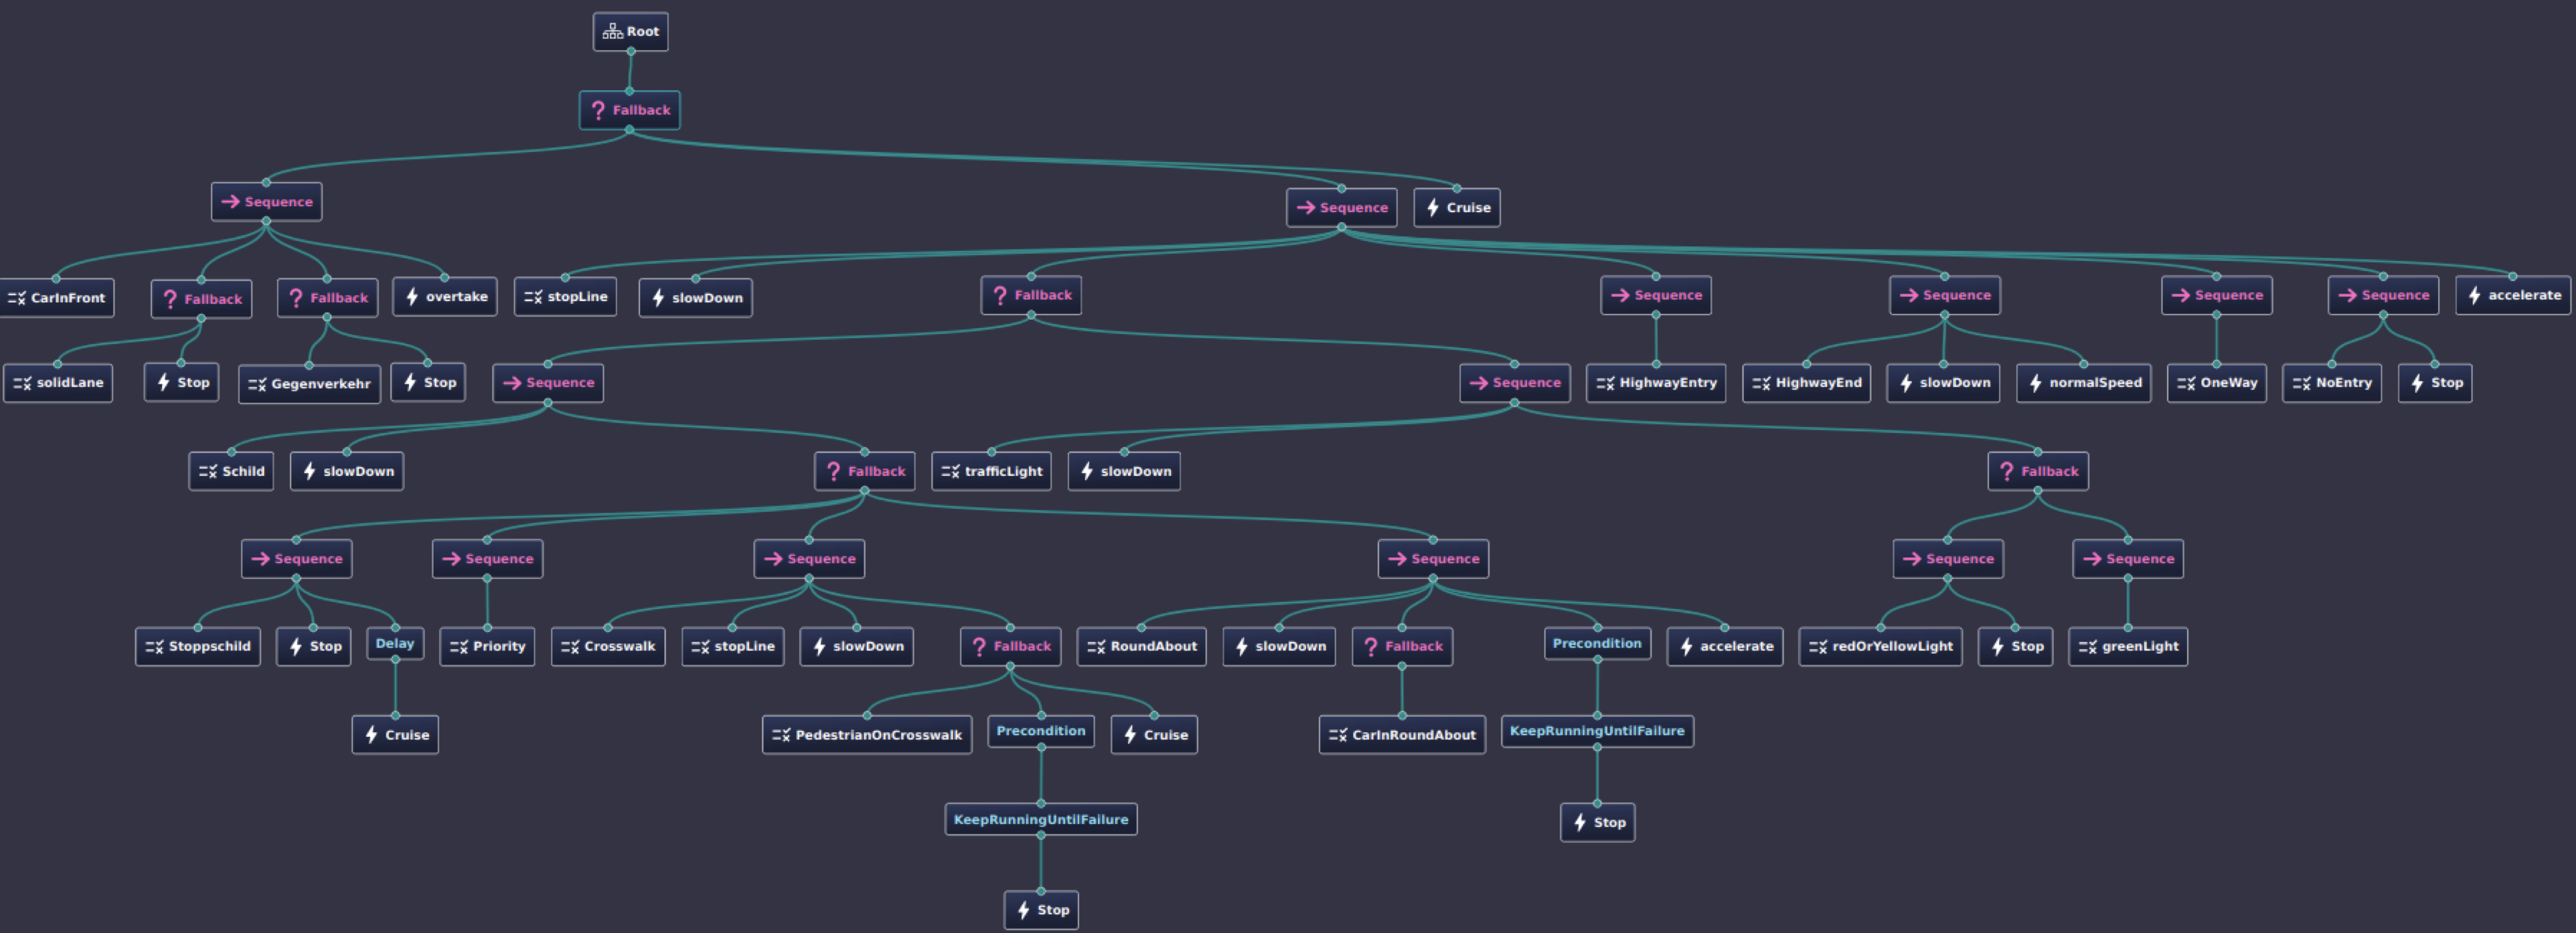
\includegraphics[width=1.4\linewidth, angle=90]{Pictures/behavior_tree_groot2.png}
    \caption{Behavior Tree für die \gls{BFMC} 2024}
    \label{fig:bt_bfmc24}
\end{figure}


